\chapter{Hypothesis testing}

\begin{definition}[Testing hypotheses]
    The hypothesis to be tested is called the null hypothesis.
 The negation of the null hypothesis is called the alternative hypothesis. The
 null and alternative hypotheses are denoted by $H_0$ and $H_1$, respectively.

 If $\theta$ denotes a population parameter, then the general format of the null
 hypothesis and alternative hypothesis is
\[
    H_0 : \theta \in \Theta_0 \quad \text{ versus } \quad H_1 : \theta \in \Theta_1 \label{eq:tst2.0} \tag{{\color{YellowOrange} $\bigstar$}}
\]

where $\Theta_0$ and $\Theta_1$ are disjoint subsets of the parameter space $\Theta$ such that

\begin{equation}
    \Theta_0 \cap \Theta_1 = \varnothing \quad \text{ and } \quad \Theta_0 \sqcup \Theta_1 \subseteq \Theta.
\end{equation}
\end{definition}

\begin{remark}
    If $\Theta_0 \cup \Theta_1 = \Theta$, then the test \eqref{eq:tst2.0} becomes
    \begin{equation}
        H_0 : \theta \in \Theta_0 \quad \text{ versus } \quad H_1 : \theta \notin \Theta_0
    \end{equation}
\end{remark}

\begin{definition}[Errors in hypothesis]
    A \textbf{type I error} is when the null hypothesis is rejected, but it is true. 
    
    A \textbf{type II error} is not rejecting null hypothesis $H_0$, but in fact $H_0$ is false.
\end{definition}

\section{What is p-value?}

One way to think of it is the courtroom example. One day you get arrested as a suspect, 
you are innocent until proven guilty.
The null hypothesis $H_0$ is that you are innocent. But now all evidence is compiled against you.
The question is: given that we are in the world where you are in fact innocent, how likely
are we to see this much evidence compiled against you? As opposed to asking ``what is the probability that you are innocent?'', that is what $p$-value means.

In statistical terminology, the $p$-value measures the "extremeness" of the sample.

\begin{definition}[p-value]
    The $p$-value is the probability we would get the sample we have or something 
    more extreme if the \textit{null hypothesis} were true.
\end{definition}

So, the smaller the $p$-value, the more evidence there is in 
the sample data against the null hypothesis and for the 
alternative hypothesis. 

So what constitutes ``sufficiently small`` and ``extreme 
enough`` to make a decision about the null hypothesis?

\section{Two sample testing}

If sample $X_1$ drawn from $N(\mu_1, \sigma^2_1)$ and is independent of 
$X_2 \sim N(\mu_2, \sigma^2_2)$, then 
\[
    X_1 - X_2 \sim N(\mu_1 - \mu_2, \sigma^2_1 + \sigma^2_2)
\]
By Central Limit theorem we obtained the result
\[
    \ols{X_1} - \ols{X_2} \sim N \left( \mu_1 - \mu_2, \frac{\sigma_1^2}{n_1} + \frac{\sigma_2^2}{n_2} \right).
\]
where $n_1$ and $n_2$ are the sample size for $X_1$ and $X_2$ correspondingly. 
Hence the test statistic is 
\begin{equation}
    z = \frac{\ols{x}_1 - \ols{x}_2 - (\mu_1 - \mu_2)}{\sqrt{\displaystyle \frac{\sigma_1^2}{n_1} + \frac{\sigma_2^2}{n_2}}}.
\end{equation}

In general, the test statistic for comparing two normal samples with known variances is as follow:
\begin{definition}[Two sample means test -- Large sample size with different variances]
    Assume that $X_1 \sim N(\mu_1, \sigma^2_1)$ and $X_2 \sim N(\mu_2, \sigma^2_2)$ are two independent samples with 
    $\sigma^2_1 \neq \sigma^2_2$. The test statistic value is
    \begin{equation}
    z = \frac{\ols{x}_1 - \ols{x}_2 - \Delta_0}{\sqrt{\displaystyle \frac{\sigma_1^2}{n_1} + \frac{\sigma_2^2}{n_2}}}.
    \end{equation}
    for null hypothesis
    \[
        H_0 : \mu_1 - \mu_2 = \Delta_0
    \]
    with all possible alternative hypotheses:

    \renewcommand{\arraystretch}{1.2}
    \begin{tabularx}{\textwidth}{|l|X|}
    \hline
    Alternative Hypothesis & Rejection Region at level $\alpha$\\
    \hline
    $H_1 : \mu_1 - \mu_2 > \Delta_0$ & $z \geq z_\alpha$ (Upper-tailed)\\
    \hline
    $H_1 : \mu_1 - \mu_2 < \Delta_0$ & $z \leq -z_\alpha$ (Lower-tailed)\\
    \hline
    $H_1 : \mu_1 - \mu_2 \neq \Delta_0$ & either $z \geq z_{\alpha/2}$ or $z \leq -z_{\alpha/2}$ (Two-tailed)\\
    \hline
    \end{tabularx}
\end{definition}

\subsection{Two samples with equal unknown population variances}

Back to previous section, the test statistic value is 
\[
    z = \frac{\ols{x}_1 - \ols{x}_2 - (\mu_1 - \mu_2)}{\sqrt{\displaystyle \frac{\sigma_1^2}{n_1} + \frac{\sigma_2^2}{n_2}}}
\]
Since $\sigma^2_1 = \sigma^2_2 = \sigma^2$, then
\[
    z = \frac{\ols{x}_1 - \ols{x}_2 - (\mu_1 - \mu_2)}{\sigma \sqrt{\displaystyle \frac{1}{n_1} + \frac{1}{n_2}}}
\]

Now both sample variances, $S^2_1$ and $S^2_2$, are estimates of $\sigma^2$. so this 
information can be combine to form a \textit{pooled} (or \textit{weighted}) estimate of variance, that is,
\[
    S^2_p = \frac{(n_1 - 1)S^2_1 + (n_2 - 1)S^2_2}{n_1 + n_2 - 2}.
\] 
Replace $\sigma^2$ with pooled variance estimator $S^2_p$, hence 
\[
    t = \frac{\ols{x}_1 - \ols{x}_2 - (\mu_1 - \mu_2)}{S_p \sqrt{\displaystyle \frac{1}{n_1} + \frac{1}{n_2}}} \sim t_{\nu=n_1+n_2-2}
\]
is a $t$-statistic with degrees of freedom given by $n_1 + n_2 - 2$.

\begin{definition}[Two sample means test -- Small sample size with equal variances]
    Assume that $X_1$ and $X_2$ are two independent samples with 
    $\sigma^2_1 = \sigma^2_2 = \sigma^2$. The test statistic value is
    \begin{equation}
    t = \frac{\ols{x}_1 - \ols{x}_2 - \Delta_0}{S_p \sqrt{\displaystyle \frac{1}{n_1} + \frac{1}{n_2}}}
    \end{equation}
    where the pooled variance id defined as
    \begin{equation}
        S^2_p = \frac{(n_1 - 1)S^2_1 + (n_2 - 1)S^2_2}{n_1 + n_2 - 2}.
    \end{equation}

    The null hypothesis is
    \[
        H_0 : \mu_1 - \mu_2 = \Delta_0
    \]
    with all possible alternative hypotheses:

    \renewcommand{\arraystretch}{1.2}
    \begin{tabularx}{\textwidth}{|l|X|}
    \hline
    Alternative Hypothesis & Rejection Region at level $\alpha$\\
    \hline
    $H_1 : \mu_1 - \mu_2 > \Delta_0$ & $t \geq t_\alpha$ (Upper-tailed)\\
    \hline
    $H_1 : \mu_1 - \mu_2 < \Delta_0$ & $t \leq -t_\alpha$ (Lower-tailed)\\
    \hline
    $H_1 : \mu_1 - \mu_2 \neq \Delta_0$ & either $t \geq t_{\alpha/2}$ or $t \leq -t_{\alpha/2}$ (Two-tailed)\\
    \hline
    \end{tabularx}
\end{definition}

\subsection{Large-Sample Test}

Assume that we have a single pooled sample of size $n_1 + n_2$ rather than having two separate samples of size $n_1$ and $n_2$.
For example, we have two different populations $X \sim BIN(n_1, p_1)$ and $Y \sim BIN(n_2, p_2)$ with $p_1 = p_2$. By combining them together 
we will have a single sample of size $n_1 + n_2$ from one population with proportion $p$, that is,
\[
    X + Y \sim BIN(n_1 + n_2, p_1 = p_2 = p)
\]

\begin{definition}[Large samples test -- difference in proportion]
    Assume that $X_1$ and $X_2$ are two populations. The large-sample test statistic is
    \begin{equation}
        z = \frac{\widehat{p}_1 - \widehat{p}_2}{\displaystyle \widehat{p}\, \widehat{q} \left(\frac{1}{n_1} + \frac{1}{n_2} \right)}.
    \end{equation}

    The null hypothesis is
    \[
        H_0 : p_1 - p_2 = 0
    \]
    with all possible alternative hypotheses:

    \renewcommand{\arraystretch}{1.2}
    \begin{tabularx}{\textwidth}{|l|X|}
    \hline
    Alternative Hypothesis & Rejection Region at level $\alpha$\\
    \hline
    $H_1 :  p_1 - p_2 > 0$ & $z \geq z_\alpha$ (Upper-tailed)\\
    \hline
    $H_1 :  p_1 - p_2 < 0$ & $z \leq -z_\alpha$ (Lower-tailed)\\
    \hline
    $H_1 :  p_1 - p_2 \neq 0$ & either $z \geq z_{\alpha/2}$ or $z \leq -z_{\alpha/2}$ (Two-tailed)\\
    \hline
    \end{tabularx}
\end{definition}


\section{Power of test}

\begin{definition}[Power of test]
    For testing null hypothesis $H_0 : \theta \in \Theta_0$, the power function 
    of a test $\phi$ with rejection region $RR$ is the function of $\theta$ defined as 
    \begin{equation}
        \beta_\phi(\theta) = \mathbb{P}_\theta[X \in RR].
    \end{equation}
\end{definition}

Note that 
\[
    \beta(\theta) = \begin{cases}
        \text{Type I error probability} & \theta \in \Theta_0\\
        \text{One minus the Type II error probability} & \theta \in \Theta^c_0\\
    \end{cases}
\]
A good test should has power value near $0$ for most $\theta \in \Theta_0$, and near $1$ for most 
$\theta \in \Theta^c_0$. The power function is similar to the MSE or risk function in
 estimation in that typically a test is better than another for some $\theta$'s but worse for other 
 $\theta$'s.

 When testing $H_0 : \theta \leq \theta_0$ with a univariate parameter $\theta$, a reasonable test 
 should have the following properties for its power function $\beta(\theta)$:

 \begin{itemize}
    \item[$\bullet$] $\beta(\theta)$ is a increasing function of $\theta$.
    \item[$\bullet$] $\lim_{n \to \theta_-} \beta(\theta) = 0$ and $\lim_{n \to \theta_+} \beta(\theta) = 1$, where 
    $\theta_-$ is the smallest $\theta$ (might be $-\infty$) and $\theta_+$ is the largest $\theta$ (might be $+\infty$).
 \end{itemize}

\subsection{Neyman-Pearson Lemma and powerful test}

\begin{lemma}[Neyman-Pearson Lemma]
    Consider we want to test $H_0 : \theta = \theta_0$ versus 
    $H_0 : \theta = \theta_1$, where $\theta_0, \theta_1$ are two distinct parameter values.

    \subsection*{Existence}
    Any test with the rejection region $\mathcal{R}$ satisfying two conditions:
    \[
        x \in \mathcal{R} \quad \text{if } f_{\theta_1}(x) > c f_{\theta_0}(x)
    \]
    \[
        x \notin \mathcal{R} \quad \text{if } f_{\theta_1}(x) < c f_{\theta_0}(x)
    \]
    for some $c \geq 0$ is a UMP test of size $\alpha_c$ with 
    \begin{equation}
        \alpha_c = \mathbb{P}_{\theta_0}[X \in \mathcal{R}].
    \end{equation}
    And note that nothing will be specified when $f_{\theta_1}(x) = c f_{\theta_0}(x)$.

    \subsection*{Uniqueness}
     If the previously specified test has a positive $c$, then every level $\alpha_c$ 
     the UMP test has size $\alpha_c$  and has the same form previously stated except
     perhaps on a set $\mathcal{A}$ satisfying
     \begin{equation}
      \mathbb{P}_{\theta_0}[\mathcal{A}] = \mathbb{P}_{\theta_1}[\mathcal{A}] = 0.
     \end{equation}
\end{lemma}
\begin{proof}
    We consider the continuous case with pdfs, and that every test can be represented 
    by the indicator function of its rejection region.

    \subsubsection*{[Existence]}
    Let $\phi(x)$ be the indicator function of the rejection region of the test in 
    the theorem and $\psi$ be the indicator function of the rejection region of any other 
    level $\alpha$ test.

    From the construction of $\phi$ we have 
    \[
        [\phi(x) - \psi(x)][f_{\theta_1}(x) - cf_{\theta_0}(x)] \geq 0 \quad \forall x \in \mathfrak{X}
    \]
    Thus,
    \begin{align*}
        0 &\leq \int_{\mathfrak{X}} [\phi(x) - \psi(x)][f_{\theta_1}(x) - cf_{\theta_0}(x)] \, \mathrm{d}x\\
        &= \beta_\phi(\theta_1) - \beta_\psi(\theta_1) - c[\beta_\phi(\theta_0) - \beta_\psi(\theta_0)]\\
        &= \beta_\phi(\theta_1) - \beta_\psi(\theta_1) - c[\alpha_c - \beta_\psi(\theta_0)]\\
        &\leq \beta_\phi(\theta_1) - \beta_\psi(\theta_1).
    \end{align*}
    This proves $\beta_\phi(\theta_1) \geq \beta_\psi(\theta_1)$.

    Since $\theta_1$ is the only point in $\Theta_0^c$, thus 
    $\phi$ is a UMP test of size $\alpha_c = \mathbb{P}_{\theta_0}[X \in \mathcal{R}]$. 

    We now further continue to proof the uniqueness part.

    \subsubsection*{[Uniqueness]}
    Let $\psi$ be the indicator function of another UMP test of level $\alpha_c$. 
    From the previous proof, we know $\phi$ is a UMP test of size $\alpha_c$ and hence 
    \[
        \beta_{\phi}(\theta_1) = \beta_{\psi}(\theta_1) 
    \]
    and 
    \[
        0 \leq \int_{\mathfrak{X}} [\phi(x) - \psi(x)][f_{\theta_1}(x) - cf_{\theta_0}(x)] \, \mathrm{d}x
        = -c[\alpha_c - \beta_\psi(\theta_0)].
    \]
    Because $c > 0$, we have $\alpha_c - \beta_\psi(\theta_0) \leq 0$.
    Since $\psi$ is a level $\alpha_c$ test, $\beta_\psi(\theta_0) \leq \alpha_c$ and hence 
    $\beta_\psi(\theta_0) = \alpha_c$. i.e. $\psi$ has size $\alpha_c$, which implies
    \[
        \int_{\mathfrak{X}} [\phi(x) - \psi(x)][f_{\theta_1}(x) - cf_{\theta_0}(x)] \, \mathrm{d}x = 0
    \]
    Now let
    \[
        \mathcal{A} := \{ x :[\phi(x) - \psi(x)][f_{\theta_1}(x) - cf_{\theta_0}(x)] > 0 \},
    \]
    then 
    \[
        \int_{\mathcal{A}} [\phi(x) - \psi(x)][f_{\theta_1}(x) - cf_{\theta_0}(x)] \, \mathrm{d}x = 0.
    \]
    We pick $h(x) = [f_{\theta_0}(x) + f_{\theta_0}(x)] / 2$, $h(x)$ is a pdf 
    and $h(x) > 0$ on $\mathcal{A}$, which is now
    \[
        \int_{\mathcal{A}} \frac{[\phi(x) - \psi(x)][f_{\theta_1}(x) - cf_{\theta_0}(x)]}{h(x)}\,h(x) \, \mathrm{d}x = 0.
    \]
    From the result we established, this become
    \[
        \mathbb{P}_h \left( \mathbb{1}_{x \in \mathcal{A}} [\phi(x) - \psi(x)][f_{\theta_1}(x) - cf_{\theta_0}(x)] = 0 \right) = 1.
    \]
\end{proof}

\begin{example}
    Suppose that $X$ represents a single observation from a population with density function
    given by
    \[
        f_X(x|\theta) = \begin{cases}
            \theta x^{\theta - 1} & \text{for } 0< x < 1\\
            0 & \text{otherwise}.
        \end{cases}
    \]
    Find the most powerful test with significance level $\alpha = 0.05$ to test
    \[
        H_0 : \theta = 2
    \]
    against the alternative
    \[
        H_1 : \theta = 1.
    \]
\end{example}
\begin{solution}
    Neyman-Pearson lemma can be applied to derive this test. In this case we comparing the 
    likelihood ratio between $H_0$ and $H_1$,
    \[
        \frac{L(\theta_0)}{L(\theta_1)} = \frac{f_X(x|\theta_0 = 2)}{f_X(x|\theta_1 = 1)}
        = \frac{2x}{1x^0} = 2x, \quad 0 < x < 1
    \]
    and the form of the rejection region for the most powerful test is 
    \[
        RR = \{ x \> | \> 2x < k \} = \left\{ x \> | \> x < \mfrac{1}{2}k \right\}
    \]
    for some constant $k$. Equivalently, $k/2$ is a constant. By letting 
    $k' = k/2$. The rejection region can be 
    simplify to
    \[
        RR = \{ x \> | \> x < k' \}.
    \]
    At significance level $\alpha = 0.05$, the value of $k'$ is determined by 
    \begin{align*}
        0.05 &= \mathbb{P}[X \in RR \> | \> \theta = 2]\\
        &= \mathbb{P}[X < k' \> | \> \theta = 2]\\
        &= \int_{0}^{k'} 2x^{2-1} \, \mathrm{d}x\\
        &= \fbox{$(k')^2$}.
    \end{align*}
    Therefore $(k')^2 = 0.05$. On solving, the rejection region of the most powerful test is actually
    \[
        RR = \{x \> | \> x < \sqrt{0.05} = 0.2236 \}.
    \]

    What is the actual value for $\textsf{power}(\theta)$ when $\theta = 1$?
    \begin{align*}
        \textsf{power}(1) &= \mathbb{P}[X \in RR \> | \> \theta = 1]\\
        &= \mathbb{P}[X < 0.2236 \> | \> \theta = 1]\\
        &= \int_{0}^{0.2236} 1 \, \mathrm{d}x\\
        &= \fbox{$0.2236$}.
    \end{align*}

    We can see that even though the rejection region gives the maximum value for $\textsf{power}(1)$ 
    among all tests with $\alpha = 0.05$. But $\beta(1) = 1 - 0.2236 = 0.7764$ is still very large.
\end{solution}

\begin{example}
    Let $X_1, X_2, X_3$ denote three independent observations from a population with pdf
    \[
        f_X(x|\theta) = \begin{cases}
            (1 + \theta) x^{\theta} & \text{for } 0\leq x \leq 1\\
            0 & \text{otherwise}.
        \end{cases}
    \]
    What is the form of the best critical region of size $0.034$ for testing 
    \[
        H_0 : \theta = 1 \quad \text{ versus } \quad H_1 : \theta = 2?
    \]
\end{example}
\begin{solution}
    By Neyman-Pearson lemma, the rejection region of the most powerful test is of the form
    \begin{align*}
        RR &= \{ (x_1, x_2, x_3) \in \mathfrak{X} \> \bigg \vert \> \frac{L(\theta_0 | x_1, x_2, x_3)}{L(\theta_1 | x_1, x_2, x_3)} \leq k \}\\
        &= \{ (x_1, x_2, x_3) \in \mathcal{I}^3 \> \bigg \vert \> \frac{\prod_{i=1}^{3} f_X(x_i|\theta_0 = 1)}{\prod_{i=1}^{3} f_X(x_i|\theta_1 = 2)} \leq k \}\\
        &= \{ (x_1, x_2, x_3) \in \mathcal{I}^3 \> | \> \frac{8 x_1 x_2 x_3}{27 x^2_1 x^2_2 x^2_3} \leq k \}\\
        &= \{ (x_1, x_2, x_3) \in \mathcal{I}^3 \> | \> \frac{1}{x_1 x_2 x_3} \leq \frac{27}{8} k \}\\
        &= \{ (x_1, x_2, x_3) \in \mathcal{I}^3 \> | \> x_1 x_2 x_3 \geq k' \}
    \end{align*}
    where $k'$ is some constant. Hence the most powerful test rejects $H_0$ is of the form 
    ``Reject $H_0$ if $x_1 x_2 x_3 \geq k'$.``
    
    The value of $k'$ is determined by the size of the test, that is, $\alpha = 0.034$.
    To evaluate the constant $k'$, we have to find the probability distribution of 
    $X_1X_2X_3$. The distribution of $X_1 X_2 X_3$ is quite challenging to get. But we have shown that 
    \[
        -2(1 + \theta) \sum_{i=1}^{3} \ln X_i \sim \chi^2_6.
    \]
    Now we proceed to find the constant $k'$. Since
    \begin{align*}
        0.034 &= \alpha \\
        &= \mathbb{P}[\text{Reject } H_0 \> | \> H_0 \text{ is true}]\\
        &= \mathbb{P}[X_1 X_2 X_3 \geq k' \> | \> \theta = 1]\\
        &= \mathbb{P}[ \ln (X_1 X_2 X_3) \geq \ln k' \> | \> \theta = 1] & \text{Taking logarithm.}\\
        &= \mathbb{P}\left[ \sum^3_{i=1} \ln X_i \geq \ln k' \> \bigg \vert \> \theta = 1\right]\\
        &= \mathbb{P}\left[ -2(1+\theta)\sum^3_{i=1} \ln X_i \geq -2(1+\theta) \ln k' \> \bigg \vert \> \theta = 1\right] & \text{ Multiply } -2(1+\theta) \text{ on both sides.}\\
        &= \mathbb{P}\left[-4 \sum_{i=1}^{3} \ln X_i \geq -4 \ln k' \right]\\
        &= \mathbb{P}\left[\chi^2_6 \geq -4 \ln k' \right]\\
    \end{align*}
    From the $\chi^2$ table, we have
    \[
        - 4 \ln k' = 1.4.
    \]
    Therefore
    \[
        k' = e^{-0.35} = \fbox{$0.7047$}.
    \]
    Thus, the most powerful test is given by ``Reject $H_0$ if $x_1 x_2 x_3 \geq 0.7047$.``

    The critical region is the region above the surface $x_1 x_2 x_3 = 0.7047$ in the unit cube $\mathcal{I}^3 = [0,1]^3$.
The following figure illustrates the rejection region.

\begin{figure}[ht]
    \centering
    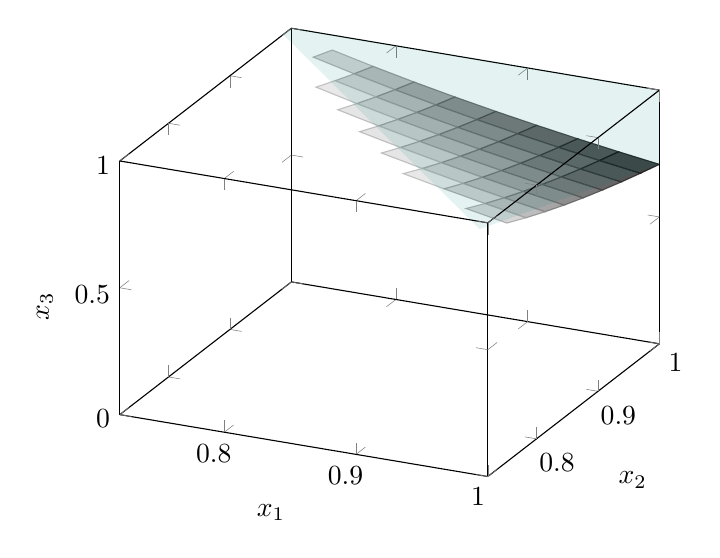
\begin{tikzpicture}
        \begin{axis}[
            3d box,
            xlabel=$x_1$, ylabel=$x_2$, zlabel=$x_1 x_2 x_3$,
            zmin=0, zmax=1,
            view={25}{30},
            zlabel=$x_3$,
            colormap/blackwhite
        ]
            \addplot3[
                surf,
                opacity=0.8,
                samples=30, samples y=30,
                domain=0.1:1, y domain=0.1:1,
                restrict z to domain=0:1
            ] { 0.7074/(x*y) };
            \fill[teal, opacity=0.1]
                (axis cs:1,1,1) -- (axis cs:0.7074,1,1) -- (axis cs:1,0.7074,1) -- (axis cs:1,1,0.7074) -- cycle;
        \end{axis}
    \end{tikzpicture}
    \caption{The rejection region is to the right of the surface $x_1 x_2 x_3 = 0.7074$.} (The shaded volume)
\end{figure}
\end{solution}

\subsection{Likelihood Ratio Test}

\begin{definition}[Likelihood Ratio Test]
    The likelihood ratio test statistic for testing $H_0 : \theta \in \Theta_0$ versus 
    $H_1 : \in \Theta^c_0$ is 
    \begin{equation}
        \Lambda(X) = \frac{\displaystyle \sup_{\theta \in \Theta_0} L(\theta | X)}{\displaystyle \sup_{\theta \in \Theta} L(\theta | X)}
    \end{equation}
    where $L(\theta|x)$ is the likelihood function based on $X = x$. A \textbf{likelihood 
    ratio test (LRT)} is any test that has a rejection region of the form 
    \[
        \{ x \> | \> \Lambda(x) \leq c \}
    \]
    where $c$ is a constant satisfying $0 \leq c \leq 1$.
\end{definition}

The logic behind LRTs is that the likelihood ratio $\Lambda(x)$ is likely to be small if there are 
parameter points in $\Theta^c_0$ for which $x$ is much more likely than for any 
parameter in $\Theta_0$. Note that in the denominator of the likelihood ratio, 
the supremum is taken over $\Theta$, not $\Theta^c_0$.

\section{Hypothesis testing for variance}

What is the likelihood ratio test of significance of size $\alpha$ for testing the null hypothesis 
\[
    H_0 : \sigma^2 = \sigma^2_0 \quad \text{ versus } \quad H_1 : \sigma^2 \neq \sigma^2_0 \, ?
\]
We illustrate the following example. 
\[
    \Theta = \{ (\mu, \sigma^2) \in \mathbb{R}^2 \> | \> -\infty < \mu < \infty, \sigma^2 > 0 \}
\]
\[
    \Theta_0 = \{ (\mu, \sigma^2) \in \mathbb{R}^2 \> | \> -\infty < \mu < \infty, \sigma^2 = \sigma^2_0 \}
\]
\[
    \Theta_1 = \{ (\mu, \sigma^2) \in \mathbb{R}^2 \> | \> -\infty < \mu < \infty, \sigma^2 \neq \sigma^2_0 \}.
\]
which $\Theta_0 \sqcup \Theta_1 = \Theta$. 

The likelihood function is given by 
\[
L(\mu, \sigma^2 | x) = \prod_{i=1}^{n} \frac{1}{\sqrt{2\pi \sigma^2}} \exp\left(-\frac{(x_i - \mu)^2}{2\sigma^2}\right)
= \bigg(\frac{1}{\sqrt{2\pi \sigma^2}}\bigg)^n \exp\left(-\frac{1}{2\sigma^2} \sum_{i=1}^{n} (x_i - \mu)^2\right).
\]
Next we find the maximum of $L(\mu, \sigma^2)$ on the set $\Theta_0$. Since the set $\Theta_0$ is equal to 
$\{ (\mu, \sigma^2_0) \in \mathbb{R}^2 \> | \> \mu \in \mathbb{R} \}$, we have 
\[
    \max_{(\mu, \sigma^2) \in \Theta_0} L(\mu, \sigma^2 | x) = \max_{\mu \in \mathbb{R}} L(\mu, \sigma^2_0 | x).
\]
From here we can see that both $L(\mu, \sigma^2 | x)$ and $\ln L(\mu, \sigma^2 | x)$ are achieving at the same value of $\mu$.
We further determine the value of $\mu$ that maximizes $\ln L(\mu, \sigma^2_0 | x)$. Taking 
the natural logarithm of the likelihood function and differentiating with respect to $\mu$, we have
\begin{align*}
    \odv{\ln L(\mu, \sigma^2_0 | x)}{\mu} &= \odv[]{}{\mu} \left[ - \frac{n}{2} \ln (\sigma^2_0) - \frac{n}{2} \ln(2\pi) - \frac{1}{2\sigma^2_0} \sum^n_{i=1} (x_i - \mu)^2 \right]\\
    &= \frac{1}{\sigma^2_0} \sum_{i=1}^{n} (x_i - \mu) \label{eq:tst1.0} \tag{{\color{red} $\heartsuit$}}
\end{align*}
Setting \eqref{eq:tst1.0} to zero and solving for $\mu$, we have
\[
    \frac{1}{\sigma^2_0} \sum_{i=1}^{n} (x_i - \mu) = 0 \implies \widehat{\mu} = \frac{1}{n} \sum_{i=1}^{n} x_i = \ols{x}.
\]
Hence, we continue to maximize $L(\ols{x}, \sigma^2_0 | x)$ with respect to $\sigma^2$. Let $\sigma^2 = \varsigma$, we have
\begin{align*}
    \odv{\ln L(\ols{x}, \varsigma | x)}{\varsigma} &= \odv[]{}{\varsigma} \left[ - \frac{n}{2} \ln (\varsigma) - \frac{n}{2} \ln(2\pi) - \frac{1}{2\sigma^2_0} \sum^n_{i=1} (x_i - \ols{x})^2 \right]\\
    &= -\frac{n}{2\varsigma} + \frac{1}{2(\varsigma)^2} \sum_{i=1}^{n} (x_i - \ols{x})^2 \label{eq:tst1.1} \tag{{\color{cyan} $\blacksquare $}}
\end{align*}
Setting the above equation \eqref{eq:tst1.1} to zero and solving for $\varsigma$, we have
\begin{align*}
    &-\frac{n}{2\varsigma} + \frac{1}{2(\varsigma)^2} \sum_{i=1}^{n} (x_i - \ols{x})^2 = 0\\
    &\implies \frac{1}{2(\varsigma)^2} \sum_{i=1}^{n} (x_i - \ols{x})^2 = \frac{n}{2\varsigma}\\
    &\implies \widehat{\varsigma} = \frac{1}{n} \sum_{i=1}^{n} (x_i - \ols{x})^2 \\
    &\implies \widehat{\varsigma} = \frac{n-1}{n} \cdot \frac{1}{n-1} \sum_{i=1}^{n} (x_i - \ols{x})^2 
    = \frac{n-1}{n} s^2.
\end{align*}
where $s^2 = \frac{1}{n-1} \sum_{i=1}^{n} (x_i - \ols{x})^2$ is the sample variance. Therefore, we obtain
\[
    \sup_{(\mu, \sigma^2) \in \Theta} L(\mu, \sigma^2 | x) = L(\ols{x}, \widehat{\varsigma} | x) 
    = \left(\frac{n}{2\pi (n-1)s^2} \right)^{n/2} \exp\left[-\frac{n}{2(n-1)s^2} \sum_{i=1}^{n} (x_i - \ols{x})^2 \right].
\]
Thus using the optimal values we found, the likelihood ratio test statistic is
\begin{align*}
    \Lambda(x_1, x_2, \ldots, x_n) &= \frac{\displaystyle \sup_{(\mu, \sigma^2) \in \Theta_0} L(\mu, \sigma^2 | x)}{\displaystyle \sup_{(\mu, \sigma^2) \in \Theta} L(\mu, \sigma^2 | x)}\\
    &= \frac{\left(\frac{n}{2\pi \sigma^2_0} \right)^{n/2} \exp\left[-\frac{1}{2 \sigma^2_0} \sum_{i=1}^{n} (x_i - \ols{x})^2 \right]}{\left(\frac{n}{2\pi (n-1)s^2} \right)^{n/2} \exp\left[-\frac{n}{2(n-1)s^2} \sum_{i=1}^{n} (x_i - \ols{x})^2 \right]}\\
    &= n^{-n/2} e^{n/2} \left(\frac{(n-1)s^2}{\sigma^2_0}\right)^{n/2} \exp\left[-\frac{1}{2} \left(\frac{1}{\sigma^2_0} - \frac{n}{(n-1)s^2}\right) \sum_{i=1}^{n} (x_i - \ols{x})^2 \right]\\
    &= n^{-n/2} e^{n/2} \left(\frac{(n-1)s^2}{\sigma^2_0}\right)^{n/2} \exp\left[ - \frac{(n-1)s^2}{2\sigma^2_0}\right] \leq k.
\end{align*}
Now this inequality can be rearranged to
\[
    \left(\frac{(n-1)s^2}{\sigma^2_0}\right)^n \exp \left[-\frac{(n-1)s^2}{\sigma^2_0}\right] \leq \left[ k \left( \frac{n}{e}^{n/2} \right) \right]^2 := K_0.
\]
where $K_0$ is some constant. Now let $H$ be a function defined by
\[
    H(w) := w^n e^{-w} \quad \text{ for } w > 0.
\]
With this notation, we see that the above inequality is equivalent to
\[
    H\left(\frac{(n-1)s^2}{\sigma^2_0}\right) \leq K_0.
\]
From this it follows that 
\[
    \frac{(n-1)s^2}{\sigma^2_0} \leq K_1 \quad \text{ or } \quad \frac{(n-1)s^2}{\sigma^2_0} \geq K_2.
\]
In view of these inequalities, the rejection region is of the form
\begin{equation}
    RR = \left\{ (x_1, x_2, \ldots, x_n) \> \bigg \vert \> \frac{(n-1)s^2}{\sigma^2_0} \leq K_1 \quad \text{ or } \quad \frac{(n-1)s^2}{\sigma^2_0} \geq K_2 \right\}
\end{equation}
and the best likelihood ratio test can be described as follows: "Reject $H_0$ if
\begin{equation}
    \frac{(n-1)s^2}{\sigma^2_0} \leq K_1 \quad \text{ or } \quad \frac{(n-1)s^2}{\sigma^2_0} \geq K_2."
\end{equation}

Since we are given the size of the test $\alpha$, the values of $K_1$ and $K_2$ can be determined. 
As the sample $X_1, X_2, \ldots, X_n$ is drawn from a normal population with mean $\mu$ and variance $\sigma^2$,
so 
\begin{equation}
    \frac{(n-1)s^2}{\sigma_0^2} \sim \chi^2_{n-1}.
\end{equation}
when the null hypothesis $H_0 : \sigma^2 = \sigma^2_0$ is true. Therefore, the likelihood ratio test of size $\alpha$ rejects $H_0$ if
\begin{equation}
    RR = \left\{ (x_1, x_2, \ldots, x_n) \> \bigg \vert \> \frac{(n-1)s^2}{\sigma^2_0} \leq \chi^2_{\frac{\alpha}{2}, n-1} \quad \text{ or } \quad \frac{(n-1)s^2}{\sigma^2_0} \geq \chi^2_{1 - \frac{\alpha}{2}, n-1} \right\}
\end{equation}
where $\chi^2_{\frac{\alpha}{2}, n-1}$ and $\chi^2_{1 - \frac{\alpha}{2}, n-1}$ are the lower and upper
$\frac{\alpha}{2}$ points of the chi-square distribution with $n-1$ degrees of freedom, respectively.

\begin{example}
    A random sample of 16 recorded deaths in the city of
 Urbana was compiled. The sample average is $71.8$ years old and the sample
 standard deviation is $9$ years. Assuming that life expectancy is
 normally distributed but with no known standard deviation,
 can we claim that the standard deviation is equal to $7$ years?
 Or is it different than that? Use a $5\%$ level of significance.
\end{example}
\begin{solution}
    We want to test 
    \[
        H_0 : \sigma^2 = 49 \quad \text{ versus } \quad H_1 : \sigma^2 \neq 49,
    \]
    where $\sigma^2$ is the variance of life expectancy in Urbana. The sample size is $n = 16$,
    and the test statistic is 
    \[
        \chi^2_0 = \frac{(16 - 1) \times 9^2}{49} = \fbox{$24.796$}.
    \]
    The corresponding critical region is 
    \[
        RR = \left\{\chi^2_0 \leq \chi^2_{0.025, 15} = 27.488 \quad \text{ or } \quad \chi^2_0 \geq \chi^2_{0.975, 15} = 6.262 \right\}.
    \]
    Hence, we do not reject $H_0$ at the $5\%$ level of significance, as 
    \[
        \chi^2_{0.975, 15} \leq \chi^2_0 \leq \chi^2_{0.025, 15}.
    \]
\end{solution}

\section*{Tutorials}

\begin{mdframed}
    \vspace{-0.25cm}
    \hspace{-0.25cm}
    \begin{Exercise}
        A firm obtains its supply of steel wire of a particular gauge from each of two 
        manufacturers $A$ and $B$. The firm suspects that the mean breaking strength, in 
        newtons (N), of wire from manufacturer $A$ differs from that supplied to 
        manufacturer $B$.

        The table below shows the breaking strengths of random samples of wire 
        \begin{center}
            \begin{tabular}{c|ccccccccc}
            A &  80.5 & 83.1 & 73.6 & 70.4 & 68.9 & 71.6 & 82.3 & 78.6 & 73.4\\
            \hline
            B &  71.4 & 86.2 & 81.4 & 72.3 & 78.9 & 80.3 & 81.4 & 78.0 & \\       
        \end{tabular}
        \end{center}

        Assuming all such breaking strengths to be normally distributed with a 
        standard deviation of 5N. Test, at the 5\% significance level, the firm's 
        suspicion.
    \end{Exercise}

    \begin{Exercise}
        A microbiologist wishes to determine whether
        there is any difference in the time it takes to
        make yoghurt from two different starters;
        lactobacillus acidophilus (A) and bulgarius (B).
        Seven batches of yoghurt were made with each
        of the starters. The table below shows the time
        taken, in hours, to make each batch.
        \begin{center}
            \begin{tabular}{c|ccccccc}
            Starter A & 6.8 & 6.3 & 7.4 & 6.1 & 8.2 & 7.3 & 6.9\\
            \hline
            Starter B & 6.1 & 6.4 & 5.7 & 5.5 & 6.9 & 6.3 & 6.7\\
        \end{tabular}
        \end{center}
        
        Assuming that both sets of times may be considered to be random samples from normal
        populations with the same variance, test the
        hypothesis that the mean time taken to make
        yoghurt is the same for both starters.
    \end{Exercise}

    \begin{Exercise}
        A new chemical process is developed for the
        manufacture of nickel-cadmium batteries. The
        company believes that this new process will
        increase the mean lifetime of a battery by 5
        hours as compared to that of batteries produced
        by the old process. Sixteen batteries produced
        by the old process were randomly selected and
        the mean and the standard deviation of the
        lifetimes of these batteries were 105.2 hours and
        9.1 hours, respectively. Fifteen batteries
        produced by the new process were also randomly
        selected and calculations gave corresponding
        values of 112.4 and 8.3 hours.

        Assuming all battery lifetimes to be normally
        distributed, test at the 5\% significance level
        whether there is
        \begin{enumerate}
            \item a difference in the variability of the two
                processes,
            \item an increase of 5 hours in the mean lifetime of
                batteries produced by the new process as
                compared to that of batteries produced by the
                old process.
        \end{enumerate}
    \end{Exercise}

    \begin{Exercise}
        What is the difference between simple and composite hypothesis?
    \end{Exercise}

    \begin{Exercise}
        If an observation $X$ is drawn from a population with probability mass function
        \[
            f_X(x|\theta) = \begin{cases}
                \mfrac{2x}{\theta^2} & \text{for } 0 \leq x < \theta\\
                0 & \text{otherwise}.
            \end{cases}
        \]
        Use Neyman-Pearson lemma to find the most powerful test for testing
        \[
            H_0 : \theta = 4 \quad \text{ versus } \quad H_1 : \theta = 5.
        \]
        Hence, find the power of the test.
    \end{Exercise}

    \begin{Exercise}
        Let $X$ be a random sample from Bernoulli distribution 
        with probability of success $\theta$. It is proposed to test
        \[
            H_0 : \theta = 0.5 \quad \text{ against } \quad H_1 : \theta = 0.3
        \]
        based on sample of size $5$.
        \begin{enumerate}
            \item Show that the rejection region for the test is 
            \[
                RR = \left\{ \sum_{i=1}^{5} X_i > 3 \right\}.
            \]
            \item Find the probabilities of type I and type II errors, as well as the power of test.
        \end{enumerate}
    \end{Exercise}

    \begin{Exercise}
        Construct the UMP test for testing 
        \[
            H_0 : \lambda = 2 \quad \text{ against } \quad H_1 : \lambda > 3
        \]
        when observations $X$ of size $n$ are drawn from population with density function
        \[
            f_X(x|\lambda) = \begin{cases}
                \displaystyle \frac{\lambda^x e^{-\lambda}}{x!} & \text{for } x = 0,1,2\ldots \\
                0 & \text{otherwise}.
            \end{cases}
        \]
        Considering level of significance $\alpha = 0.02$.
    \end{Exercise}

    \begin{Exercise}
        Find the likelihood ratio test for testing $H_0:\mu = \mu_0$ versus 
        $H_1:\mu \neq \mu_0$ when a random sample is drawn from 
        $N(\mu, 625)$.
    \end{Exercise}

    \begin{Exercise}
        The daily output of 9 randomly selected operators was recorded before and after a two-week 
        training programme:

        \begin{center}
            \begin{tabular}{c|ccccccccc}
                Operator & A & B & C & D & E & F & G & H & I\\
                \hline
                Before & 52 & 72 & 58 & 55 & 67 & 63 & 56 & 69 & 57\\
                After & 50 & 90 & 62 & 56 & 80 & 72 & 58 & 84 & 60\\
            \end{tabular}
        \end{center}

        Assuming the change in the daily output follows a normal distribution, examine the 
        hypothesis that the two-week training programme results in a significant increase in the 
        mean daily output of the operators at the 5\% significance level.
    \end{Exercise}
\end{mdframed}